%%%%%%%%%%%%%%%%%%% - ANEXOS - %%%%%%%%%%%%%%%%%%%

\newpage
\section*{ANEXOS} \label{sec:anexos} % Se añade un asterisco a \section para que el título no esté numerado.
\addcontentsline{toc}{section}{ANEXOS} % Al utilizar \section* se ha de añadir manualmente el apartado al índice (Table Of Contents, TOC).
\markright{ANEXOS} % Al utilizar \section* se ha de añadir manualmente el título del apartado al encabezado.

\renewcommand{\thesubsection}{\Alph{subsection}} % Se numeran los anexos con letras del alfabeto en lugar de números.
% Se indica que las tablas, figuras y códigos se numeran con el código del anexo (A, B, C, ...) seguido del número de tabla, figura o código dentro del anexo (tabla A.2, figura C.1, etc.)
\renewcommand{\thetable}{\Alph{subsection}.\arabic{table}}
\renewcommand{\thefigure}{\Alph{subsection}.\arabic{figure}}

% ---------------- Primer anexo ---------------- %
\setcounter{subsection}{0}
\setcounter{table}{0}
\setcounter{figure}{0}
\subsection{Anexo I: Guión de la práctica de seguimiento de carga} \label{sec:anexo1}

\begin{itemize}
    \item \textbf{Título:} Simulación de una maniobra de seguimiento de carga de un \acrshort{smr} con el \acrshort{sgiz}.
    \item \textbf{Duración aproximada:} 2 horas.
    \item \textbf{Lugar de realización:} \acrfull{sgiz} de la Escuela Técnica Superior de Ingenieros Industriales (UPM).
    \item \textbf{Impartición:} Alumnos de la asignatura de \textit{Tecnologías Avanzadas en Reactores Nucleares} del \textit{Máster en Ciencia y Tecnología Nuclear}.
\end{itemize}

\subsubsection{Introducción}

Tradicionalmente, por razones técnicas y económicas, las centrales nucleares se han empleado para la generación de energía eléctrica como \textbf{centrales base}.
Sin embargo, últimamente ha aumentado el interés en la capacidad de seguimiento de carga de las plantas nucleares, principalmente, en los siguientes dos casos concretos:

\begin{itemize}
  \item \textbf{Redes eléctricas donde la energía nuclear representa una gran parte de la generación energética total} e interesa que esta fuente de energía, al ser mayoritaria, pueda adaptarse a las fluctuaciones de la demanda eléctrica.
  \item \textbf{Redes eléctricas donde las fuentes de energía renovable intermitentes ---como la solar y la eólica--- constituyen una parte importante de la producción eléctrica total} y presentan importantes variaciones en la producción.
\end{itemize} 

Los \textbf{\acrfullpl{smr}}, debido a la incorporación de técnicas de modulación de potencia mejoradas y al diseño de sistemas de control avanzados, tienen mejores capacidades de seguimiento de carga, lo cual los hace muy adecuados para operar junto con fuentes de energía renovable intermitentes. En concreto, los niveles de potencia de los pequeños reactores modulares pueden variar entre el \textbf{15 - 100 \%}, con rampas de potencia típicas de \textbf{2 - 5 \%/min}, logrando rampas de potencia de \textbf{10 - 20 \%/min} en algunos diseños (\cite{ANS_2019}): 

\begin{table}[h]
  \centering
  \resizebox{0.75\textwidth}{!}{%
  \begin{tabular}{|
    >{\columncolor[HTML]{FFCCC9}}c |c|c|c|}
    \hline
    \cellcolor[HTML]{ECF4FF}\begin{tabular}[c]{@{}c@{}}Tipo de\\ SMR\end{tabular} &
      \cellcolor[HTML]{ECF4FF}\begin{tabular}[c]{@{}c@{}}Potencia eléctrica\\ (MWe)\end{tabular} &
      \cellcolor[HTML]{ECF4FF}\begin{tabular}[c]{@{}c@{}}Rango de potencia\\ (\%)\end{tabular} &
      \cellcolor[HTML]{ECF4FF}\begin{tabular}[c]{@{}c@{}}Rampa de potencia\\ (\%/min)\end{tabular} \\ \hline
    \textit{\begin{tabular}[c]{@{}c@{}}Pressurized Water Reactor\\ (\acrshort{pwr})\end{tabular}}             & 50 - 160   & 20 - 100 \% & 2 - 5 \\ \hline
    \textit{\begin{tabular}[c]{@{}c@{}}Molten Salt Reactor\\ (\acrshort{msr})\end{tabular}}                   & 37,5 - 192 & 20 -100 \%  & 5     \\ \hline
    \textit{\begin{tabular}[c]{@{}c@{}}High Temperature Gas-cooled \\ Reactor (\acrshort{htgr})\end{tabular}} & 76 - 286   & 15 - 100 \% & 5     \\ \hline
    \textit{\begin{tabular}[c]{@{}c@{}}Lead-cooled Fast Reactor\\ (\acrshort{lfr})\end{tabular}}              & 3 - 450    & 0 - 125 \%  & 10    \\ \hline
    \textit{\begin{tabular}[c]{@{}c@{}}Sodium Fast Reactor\\ (\acrshort{sfr})\end{tabular}}                   & 50 - 311   & 20 - 100 \% & 1 - 2 \\ \hline
    \textit{\begin{tabular}[c]{@{}c@{}}Heat Pipe cooled Reactor\\ (\acrshort{hpr})\end{tabular}}              & 0,2 - 25   & 60 - 100 \% & 20    \\ \hline
    \end{tabular}
  }
  \caption{Capacidad de seguimiento de carga de 16 diseños distintos de \acrshortpl{smr} agrupados en el tipo de SMR al que pertenece cada diseño (\cite{ANS_2019}).}
  \label{tab:capacidad_seguimiento_de_carga_smrs2}
  \end{table}
  
  \subsubsection{Fundamentos teóricos}

  Es importante tener en cuenta que las maniobras de variación de potencia se realizan de acuerdo con el criterio \textit{\textbf{reactor sigue a turbina}}, por lo que se actúa sobre la turbina y no directamente sobre el reactor. La potencia que suministra la turbina depende del gasto másico de vapor y del salto entálpico ---que, a su vez, depende de las condiciones termodinámicas del vapor a la entrada y a la salida de la turbina---. Por tanto, para variar la potencia es necesario modificar el gasto de vapor, lo cual se realiza actuando sobre las válvulas de regulación de la turbina. Estas, se abren o se cierran ---dejando pasar un mayor o menor gasto de vapor--- según se quiera aumentar o reducir la potencia, respectivamente (\cite{apuntes_centrales}). Como consecuencia de esta maniobra, se producen cambios en otras magnitudes, que serán las señales de actuación sobre distintos sistemas de control, que procurarán acomodar la planta a la nueva situación mediante los siguientes mecanismos:

\begin{itemize}
  \item \underline{Variación en la concentración de ácido bórico:} Se emplea en los reactores \acrshort{pwr} y el principal problema de este mecanismo es que se trata de un proceso lento que requiere de varios minutos para tener efecto.
  
  \item \underline{Empleo de bancos de control u operación de las barras de control:} 
  Se trata, concretamente, de los bancos de barras de control A, B, C y D ---en Zorita, los bancos A y B---. Las ventajas que presenta el empleo de las barras de control es que ofrecen una respuesta rápida y pueden adaptarse a sistemas de control automático. Sin embargo, producen una distorsión en la distribución de potencia, ya que se agota más el combustible en la parte inferior del reactor que en la parte superior, por donde se insertan dichas barras en el caso de los \acrshortpl{pwr}. Este problema puede corregirse variando la concentración de ácido bórico y retirando después las barras de control.

  \item \underline{Empleo del coeficiente de temperatura del moderador:} Este coeficiente representa la variación de la \gls{reactividad} con la temperatura del moderador: 
  
  \begin{equation}
    \alpha_{mod}=\frac{\partial \rho}{\partial T_{mod}}
  \end{equation}

  Un reactor, para ser intrínsecamente estable debe tener un coeficiente de potencia negativo, de modo que un aumento en la reactividad del núcleo conlleve una reducción de la potencia:

  \begin{equation} \label{coeficiente_potencia2}
    \frac{\partial \rho}{\partial P}=\frac{\partial \rho}{\partial T_c} \frac{\partial T_c}{\partial P}+\frac{\partial \rho}{\partial T_{\mathrm{mod}}} \frac{\partial T_{\mathrm{mod}}}{\partial P}=\alpha_{T c} \frac{\partial T_c}{\partial P}+\alpha_{\mathrm{mod}} \frac{\partial T_{\mathrm{mod}}}{\partial P}<0
  \end{equation}

  Para ello, es necesario que el coeficiente Doppler ($\alpha_{T_{c}}$) y el coeficiente de temperatura del moderador ($\alpha_{mod}$) sean negativos. En un reactor submoderado con coeficiente de temperatura del moderador negativo, un aumento de temperatura del moderador conlleva una disminución de la \gls{reactividad} y, por la ecuación \ref{coeficiente_potencia2}, una consecuente disminución de la potencia. De esta manera, aumentando la temperatura del moderador o sobrerrefrigerando el núcleo se disminuye o aumenta, respectivamente, la potencia de la planta (\cite{apuntes_centrales}).
  
  Las ventajas que presenta este método es que no hace uso de materiales que puedan desgastarse y que proporciona una potencia homogénea en todo el reactor. Sin embargo, si los cambios de potencia ---y, por tanto, de temparatura--- son muy bruscos, será necesario un presionador lo suficientemente grande como para adaptar la presión del circuito primario a los cambios del nivel de agua producidos (\cite{seguimiento_carga_josep_rey}).
\end{itemize}

\subsubsection{Objetivo de la simulación}

El objetivo de esta práctica es simular una maniobra de seguimiento de carga con el fin de adaptarse a las fluctuaciones de la energía eólica y solar en un período de tiempo concreto. Una vez realizada la simulación, el simulador ofrece las gráficas y tablas de datos necesarias para analizar el funcionamiento de la planta durante ese modo de operación. Por último, debido a que la Central Nuclear de Zorita es de un solo lazo y produce 150 MWe de potencia ---características típicas de algunos \acrshortpl{smr}---, se pretende analizar la capacidad de seguimiento de carga de esta central y compararla con la que puede tener un \acrshort{smr}.

\subsubsection{Contextualización}

El caso concreto en el que se contextualiza la simulación es una tarde de agosto muy soleada y con muy poco viento en la que, a las 20.00, llegan de repente fuertes vientos a la península y la producción eólica aumenta drásticamente. La central baja en unos 15 minutos la producción de potencia al 50\% y, tras permanecer unos 10 minutos a dicho nivel de producción, comienza a atardecer a las 20.30, disminuyendo rápidamente la producción solar. Ante esto, la central vuelve a subir ---en otros 15 minutos aproximadamente--- la potencia hasta el 100\%, nivel de producción al que se mantendrá toda la noche debido a la falta de producción solar.

\subsubsection{Procedimiento} \label{procedimiento}

Dado que en esta simulación se trabajará con valores de potencia dentro del rango entre el 15 - 100 \%\footnote{Por debajo del 15\% de potencia, las actuaciones deberían hacerse en \textit{modo manual}.}, la central trabajará en \textit{modo automático}. En este modo, el sistema de control del reactor permite a la central adaptarse automáticamente a variaciones de potencia del \textbf{3\% por minuto} y a cambios bruscos del 5\% (ritmos superiores supondrían un elevado estrés térmico). 

Durante toda la simulación es importante \textbf{comprobar que la diferencia entre la temperatura media del primario ($T_{med}$) y la temperatura de referencia\footnote{Temperatura teórica que determina, para cada caudal de vapor, la temperatura media que debería haber en el primario para que la potencia nuclear se adapte a la potencia demandada por la turbina.} ($T_{ref}$) es inferior a 2ºC}, asegurando así el funcionamiento estable del reactor. En caso de que en algún momento no se cumpla este requisito, disminuir ligeramente la tasa de variación de potencia.

A continuación se detallan los pasos a seguir en el transcurso de la simulación:

\begin{enumerate}
  \item Una vez encendido y ejecutado el simulador, cargar la condición inicial 51: \textit{100\% BOL nuevos coeficientes de reactividad}.
  
  \item Los sistemas involucrados en un transitorio de variación de carga son, principalmente, el circuito primario y el secundario. Por tanto, es suficiente con abrir las siguientes dos pantallas:
  \begin{itemize}
    \item \textbf{Pantalla NSSS-SI-AFW:} Circuito primario. Principales componentes de interés: lazo del primario, reactor, presionador (PZR) y generador de vapor (GV).
    \item \textbf{Pantalla MS-MSR-GS-TU-OPC-LO:} Circuito secundario. Principales componentes de interés: controlador del límite de carga y válvulas de regulación (1, 2, 3 y 4).
    \end{itemize}

  \begin{figure}[h]
    \centering
    \includegraphics[width=0.75\textwidth]{content/figures/pantallas_simulacion1.png}
    \caption{Pantallas necesarias para la simulación. Los valores de la pantalla superior corresponden al momento inicial de la simulación y, los de la inferior, a una fase intermedia de la misma.}
    \label{fig:pantallas_simulacion1}
  \end{figure}

  \item Iniciar la simulación y comenzar las bajadas de potencia pulsando ``BAJAR'' en el controlador del límite de carga en la pantalla MS-MSR-GS-TU-OPC-LO. Realizar \textbf{bajadas del 3\%} en turbina y \textbf{esperar 1 minuto y medio} para que se estabilice el sistema en cada una de ellas. 
  \item Realizar el proceso anterior de bajada hasta alcanzar el \textbf{50\% de potencia nuclear}. Una vez llegados a este punto, mantener el nivel de potencia durante 10 minutos.
  \item Pasados los 10 minutos de estabilización, realizar las necesarias subidas de potencia pulsando el botón ``SUBIR'' del controlador del límite de carga. Igual que en el paso 3, realizar \textbf{subidas del 3\%} en turbina y \textbf{esperar 1 minuto y medio} tras cada una de ellas.
  \item Una vez alcanzado el \textbf{100\% de potencia nuclear}, esperar 2 minutos para que se estabilice el sistema y finalizar la simulación.
\end{enumerate}  

\subsubsection{Resultados y cuestiones}

\begin{enumerate}
  \item Emplear la funcionalidad \textit{Gráfico de tendencias} del simulador para tabular y graficar los siguientes parámetros en función del tiempo de la operación:
    \begin{itemize}
      \item \underline{Gráfica 1 - Variaciones de potencia}
      \begin{itemize}
        \item Potencia nuclear
        \item Potencia activa del generador principal
      \end{itemize}
      \item \underline{Gráfica 2 - Variaciones de temperatura}
      \begin{itemize}
        \item Temperatura media
        \item Temperatura de referencia
      \end{itemize}
      \item \underline{Gráfica 3 - Posición del las válvulas de control de la turbina}
      \begin{itemize}
        \item Posición de la válvula de control 1
        \item Posición de la válvula de control 2
        \item Posición de la válvula de control 3
        \item Posición de la válvula de control 4
      \end{itemize}
      \item \underline{Gráfica 4 - Caudal de vapor}
      \item \underline{Gráfica 5 - Inserción de las barras de control}
      \begin{itemize}
        \item Pasos extraídos del banco de control 1
        \item Pasos extraídos del banco de control 2
      \end{itemize}
      \item \underline{Gráfica 6 - Concentración de boro}
      \item \underline{Gráfica 7 - Parámetros del presionador}
      \begin{itemize}
        \item Presión del presionador
        \item Nivel del presionador 
        \item Caudal de descarga
      \end{itemize}
      \item \underline{Gráfica 8 - Parámetros del generador de vapor}
      \begin{itemize}
        \item Presión del generador de vapor
        \item Nivel del generador de vapor (rango estrecho)
        \item Presión de la cámara de impulsos
      \end{itemize}
    \end{itemize}
  
  \item Responder a las siguientes cuestiones sobre las gráficas previamente obtenidas:
  \begin{itemize}
    \item \underline{Cuestión gráficas 1 y 2:} ¿A qué se deben los ligeros picos de potencia que se dan en la curva de \textit{potencia nuclear}? ¿Tienen alguna relación con los picos que se dan en la curva de \textit{temperatura media}?
    \item \underline{Cuestión gráfica 5:} ¿A qué parámetro físico del reactor responde el sistema de control automático cuando inserta o extrae las barras de control?
    \item \underline{Cuestión gráfica 6:} A parte de aportar reactividad negativa cuando es necesario, pese al inconveniente de su lentitud, ¿qué ventaja presenta la inyección de ácido bórico para apoyar en las variaciones de potencia?
    \item \underline{Cuestión gráficas 7 y 8:} Razonar en un breve párrafo el comportamiento de los distintos parámetros graficados del generador de vapor y del presionador.
  \end{itemize}

  \item Completar la tabla \ref{tab:resultados_simulacion1} y, tras observar la tabla \ref{tab:capacidad_seguimiento_de_carga_smrs2} y las figuras \ref{fig:seguimiento de carga_smr} y \ref{fig:sim2_potencias}, contestar a la siguiente cuestión:
  \begin{itemize}
    \item \underline{Cuestión \acrshortpl{smr}:} ¿Se puede decir que la capacidad de seguimiento de carga de la Central Nuclear de Zorita es similar a la de algunos \acrshortpl{smr}?
  \end{itemize}
  \begin{table}[h]
    \centering
    \vspace{-0.5cm}
    \resizebox{1\textwidth}{!}{%
    \begin{tabular}{|c|c|c|c|c|c|c|}
      \hline
      \rowcolor[HTML]{ECF4FF} 
      \textbf{\begin{tabular}[c]{@{}c@{}}Potencia inicial\\ (MWe generados\\  y \% nuclear)\end{tabular}} &
        \textbf{\begin{tabular}[c]{@{}c@{}}Potencia intermedia\\ (MWe generados\\  y \% nuclear)\end{tabular}} &
        \textbf{\begin{tabular}[c]{@{}c@{}}Duración bajada\\ de potencia\\ (min)\end{tabular}} &
        \textbf{\begin{tabular}[c]{@{}c@{}}Rampa media de \\ potencia en la bajada\\ (\%/min)\end{tabular}} &
        \textbf{\begin{tabular}[c]{@{}c@{}}Potencia final\\ (MWe generados\\  y \% nuclear)\end{tabular}} &
        \textbf{\begin{tabular}[c]{@{}c@{}}Duración subida\\ de potencia \\ (min)\end{tabular}} &
        \textbf{\begin{tabular}[c]{@{}c@{}}Rampa media de \\ potencia en la subida \\ (\%/min)\end{tabular}} \\ \hline
      \cellcolor[HTML]{FFFFFF}\textit{} &
         &
         &
         &
         &
         &
         \\ \hline
      \end{tabular}
    }
    \caption{Principales resultados de la maniobra de seguimiento de carga.}
    \label{tab:resultados_simulacion1}
    \end{table}

    \begin{figure}[h]
      \centering
      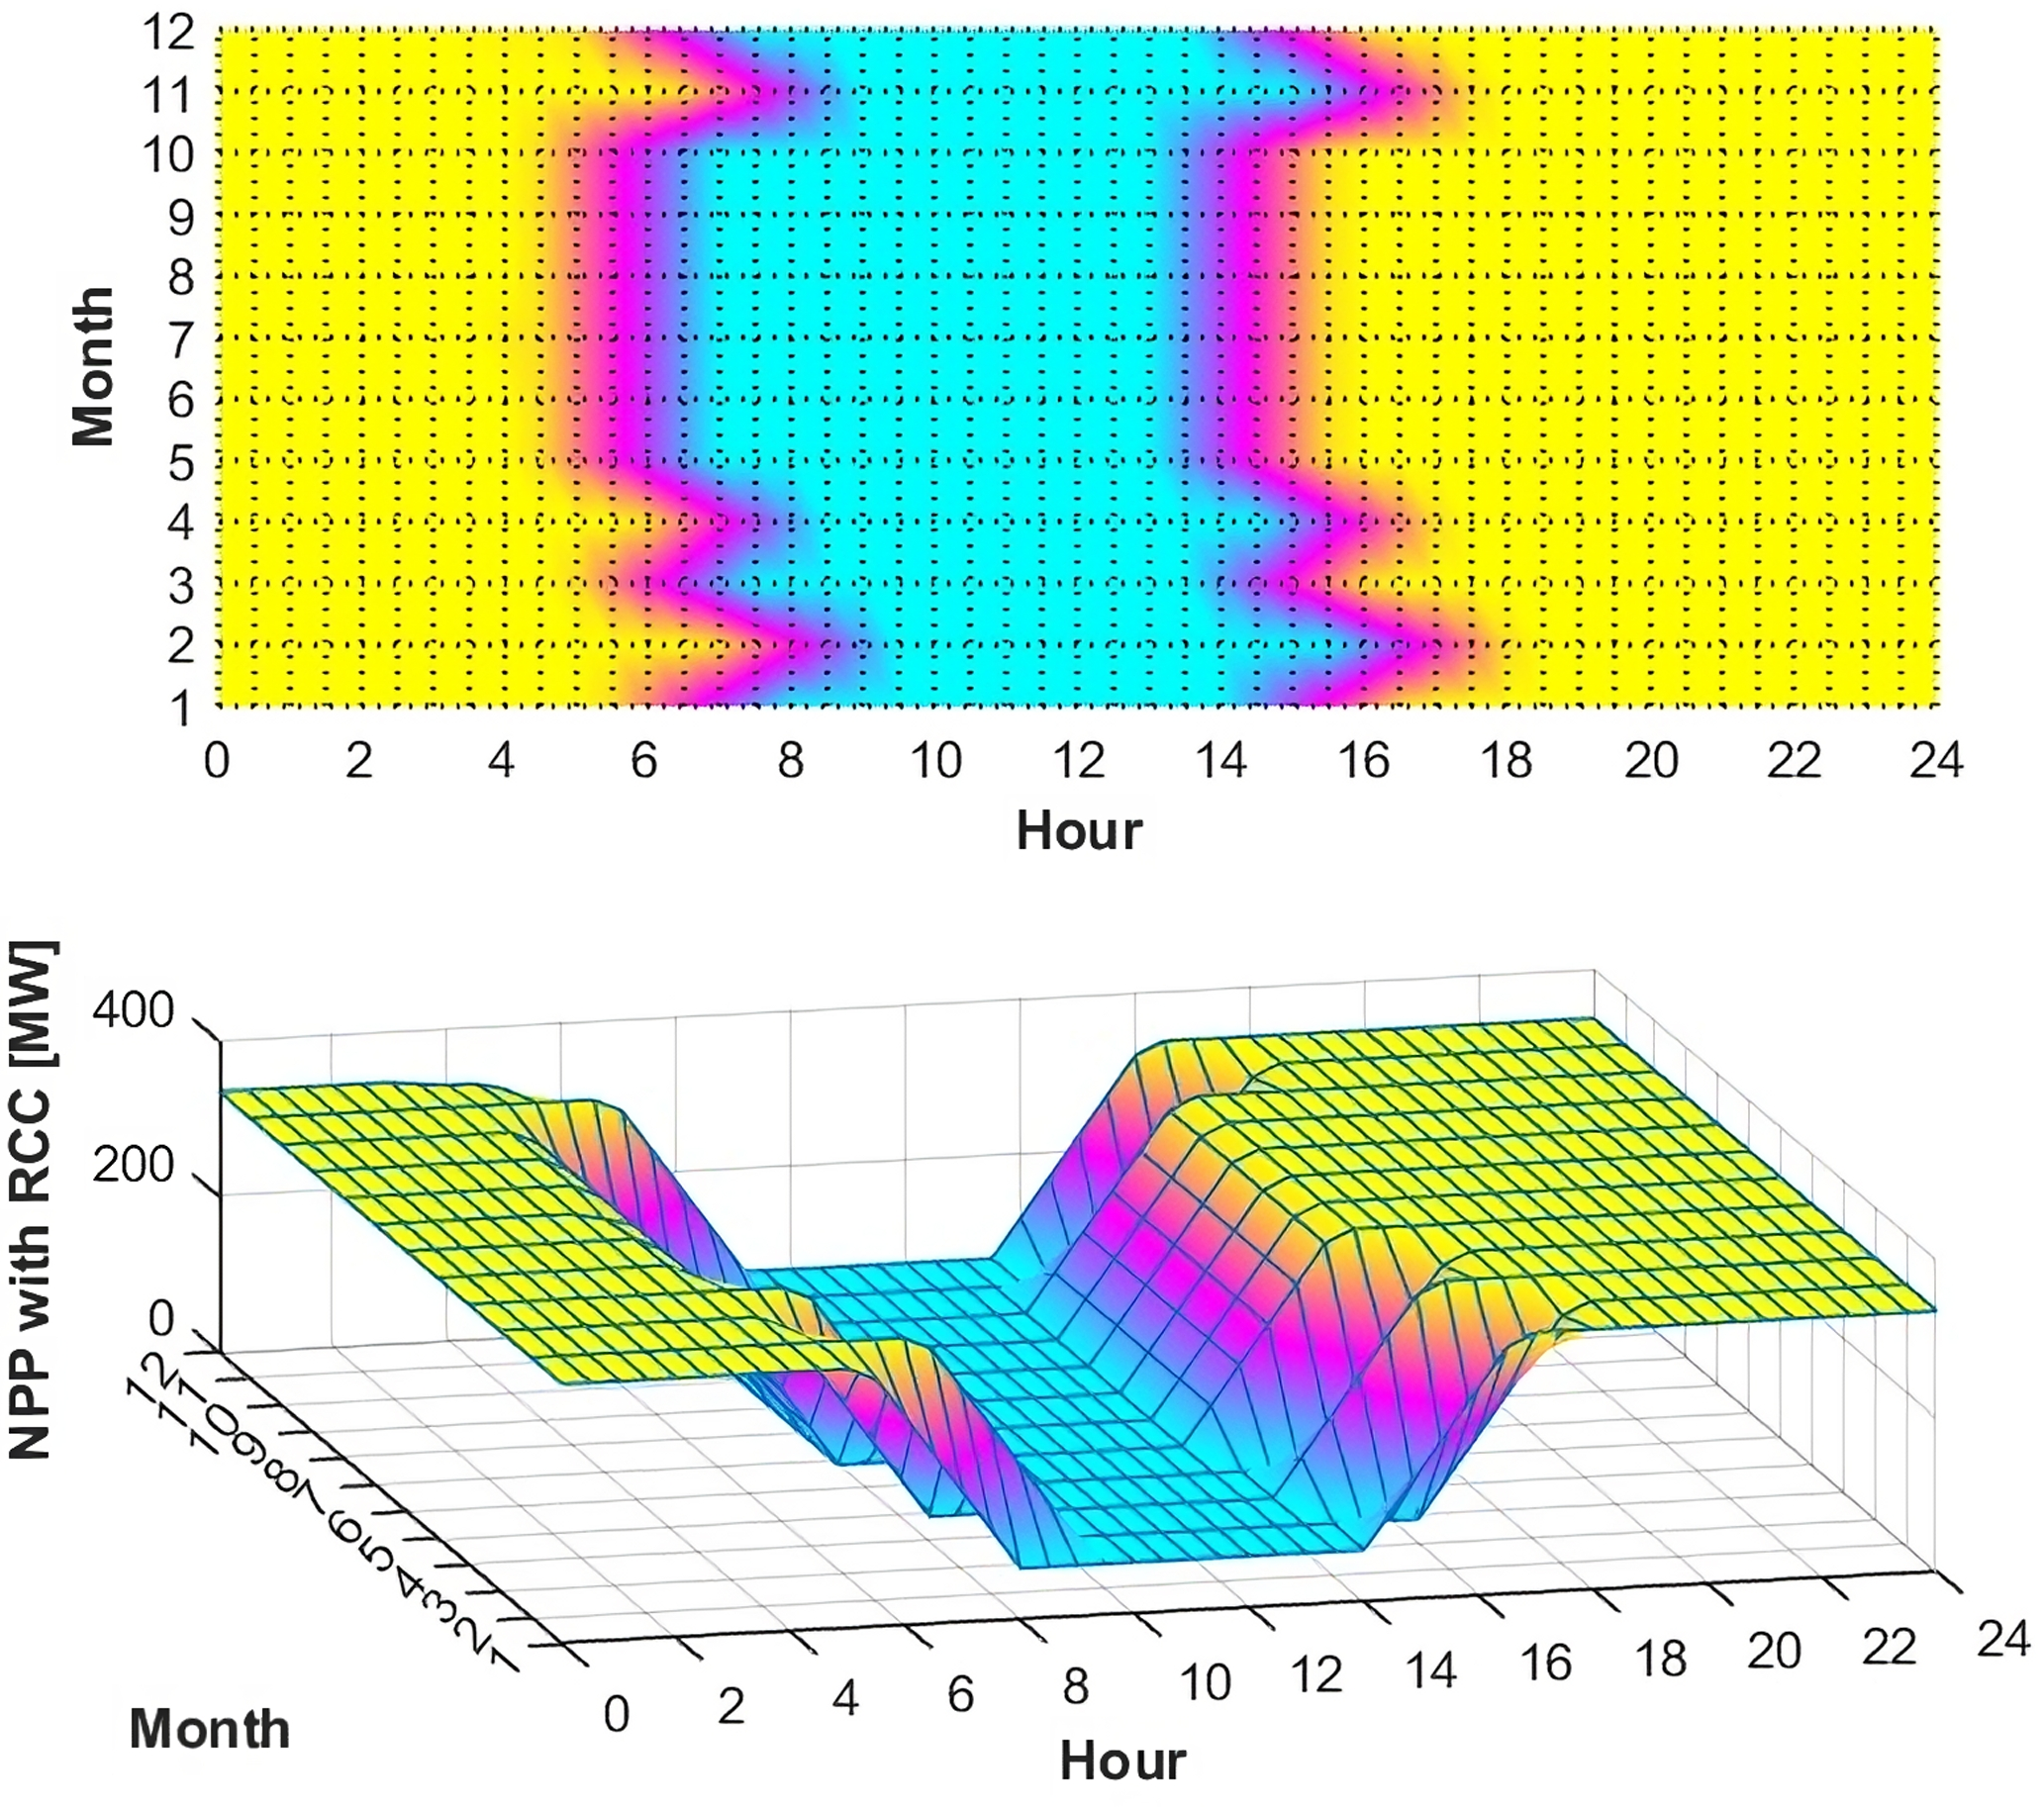
\includegraphics[width=0.62\textwidth]{content/figures/seguimiento_carga_smr.png}
      \vspace{-0.1cm}
      \caption{Estudio del seguimiento de carga (100 - 20 - 100\%) de un \acrshort{smr} de 335 MWe, adaptándose a las horas de máxima producción solar de los distintos meses del año en Seúl. Tasa de variación de carga: 1,25\%/min. \textbf{Color amarillo} = máxima potencia (335 MWe). \textbf{Color azul} = 67 MWe (20\% de potencia). \textbf{Color violeta} = rampas de potencia (\cite{SMRs_load_following_PV}).}
      \label{fig:seguimiento de carga_smr}
    \end{figure} 

    \begin{figure}[h!]
      \centering
      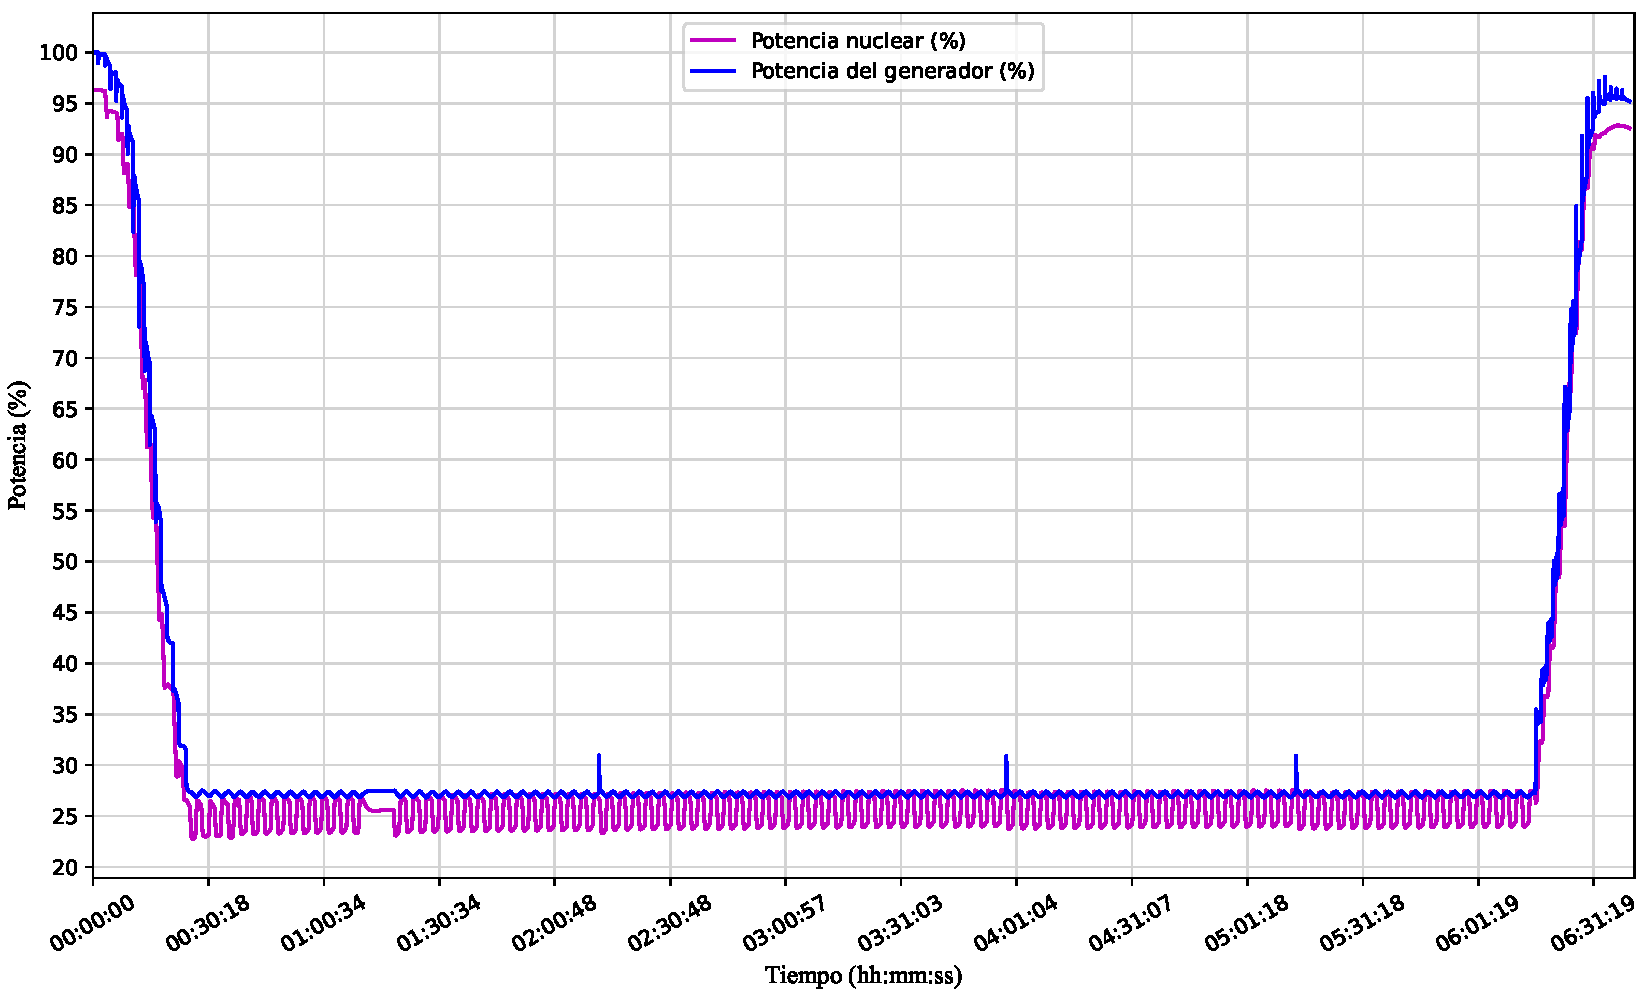
\includegraphics[width=0.96\textwidth]{content/figures/sim2_potencias_arreglo.pdf}
      \vspace{-0.3cm}
      \caption{Variación de potencias en una maniobra de  seguimiento de carga (100 - 25 - 100\%) de 6 horas y 40 minutos realizada en el \acrshort{sgiz} simulando la adaptación a las horas de máxima producción solar de un día de invierno. Tasa de variación de carga empleada: 3\%/min.}
      \label{fig:sim2_potencias}
    \end{figure}
\end{enumerate}

\subsubsection{Respuestas a las cuestiones planteadas}

A continuación se muestran las gráficas obtenidas en la simulación, junto con las respuestas a las cuestiones planteadas. El objetivo de las cuestiones es apoyar el análisis de las gráficas. 

\begin{figure}[!h]
  \centering
  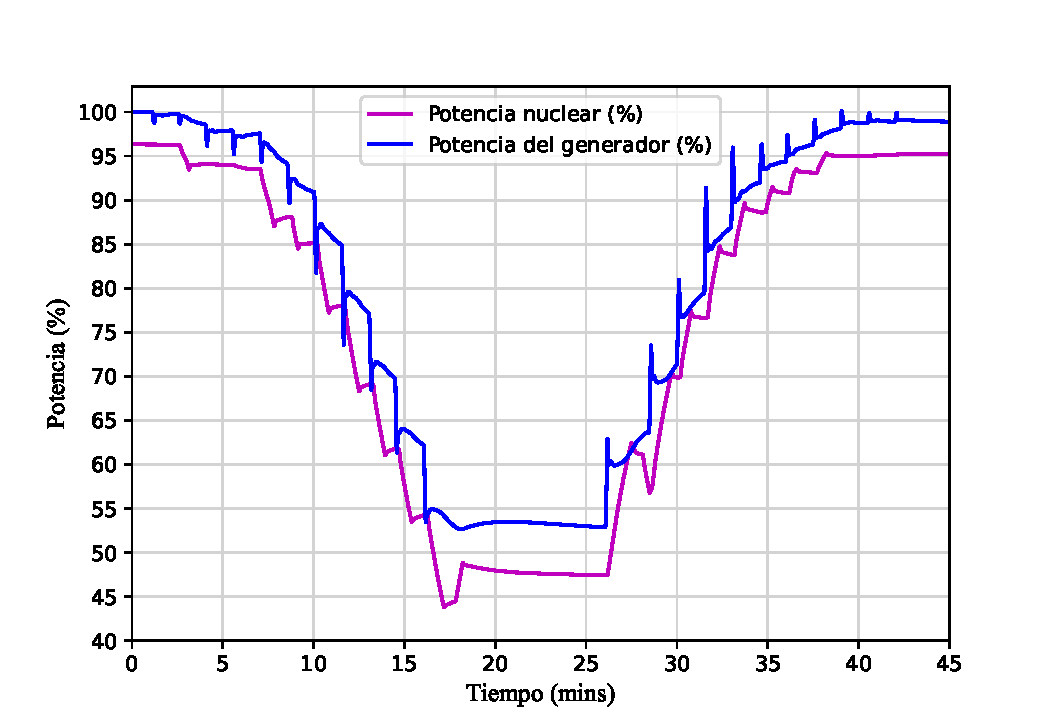
\includegraphics[width=0.75\textwidth]{content/figures/sim1_potencias.pdf}
  \vspace{-0.3cm}
  \caption{\textit{Gráfica 1} - Variaciones de potencia.}
  \label{fig:sim1_potencias}
\end{figure}

\begin{figure}[h]
  \centering
  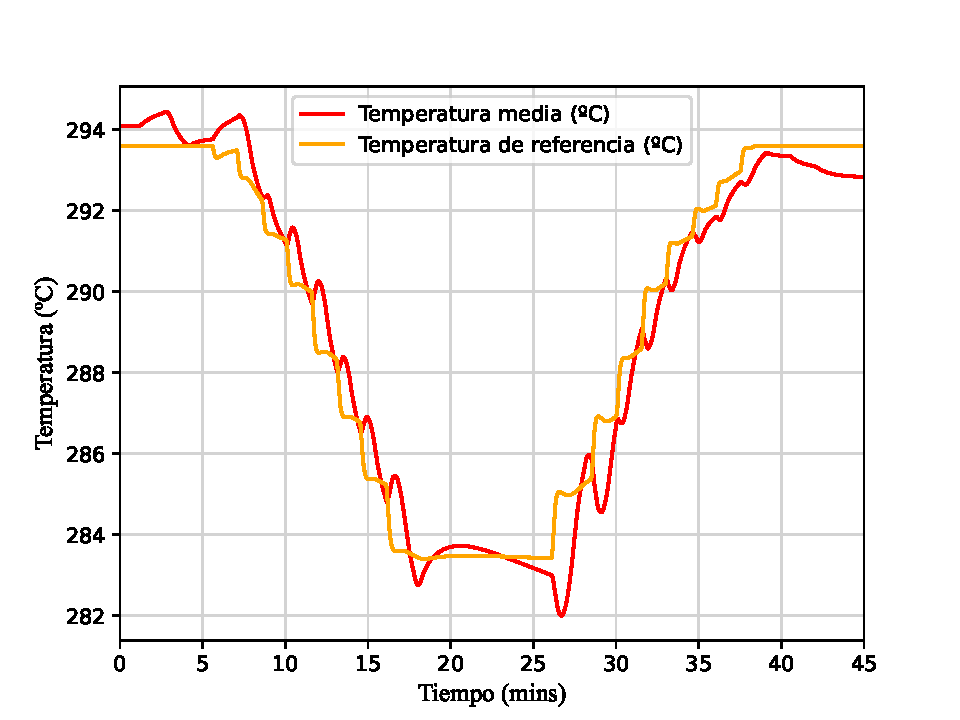
\includegraphics[width=0.75\textwidth]{content/figures/sim1_temperaturas.pdf}
  \vspace{-0.3cm}
  \caption{\textit{Gráfica 2} - Variaciones de temperatura.}
  \label{fig:sim1_temperaturas}
\end{figure}

\underline{Cuestión gráficas 1 y 2:} Al cerrar las válvulas de control de la turbina para disminuir la potencia, se reduce el gasto de vapor y el foco frío de la planta se hace menos eficiente. Esto provoca ``saturaciones'' en el circuito primario que originan picos de aumento de temperatura. Como el coeficiente de temperatura del moderador es negativo, estos aumentos de temperatura conllevan picos de disminución de la potencia. Cuando se aumenta la potencia en la turbina sucede lo contrario. Cabe destacar que estos picos se amplifican cuando trabajamos a potencias bajas ---en este caso, alrededor del 50\%--- ya que se trata de una zona de menor estabilidad para el sistema de control del reactor.

\underline{Observación adicional:} La \textit{gráfica 1} muestra perfectamente el comportamiento \textit{reactor sigue a turbina}. Primero disminuye la potencia de la turbia y, pasados unos instantes, disminuye la potencia nuclear, y así sucesivamente.

\begin{figure}[!h]
  \centering
  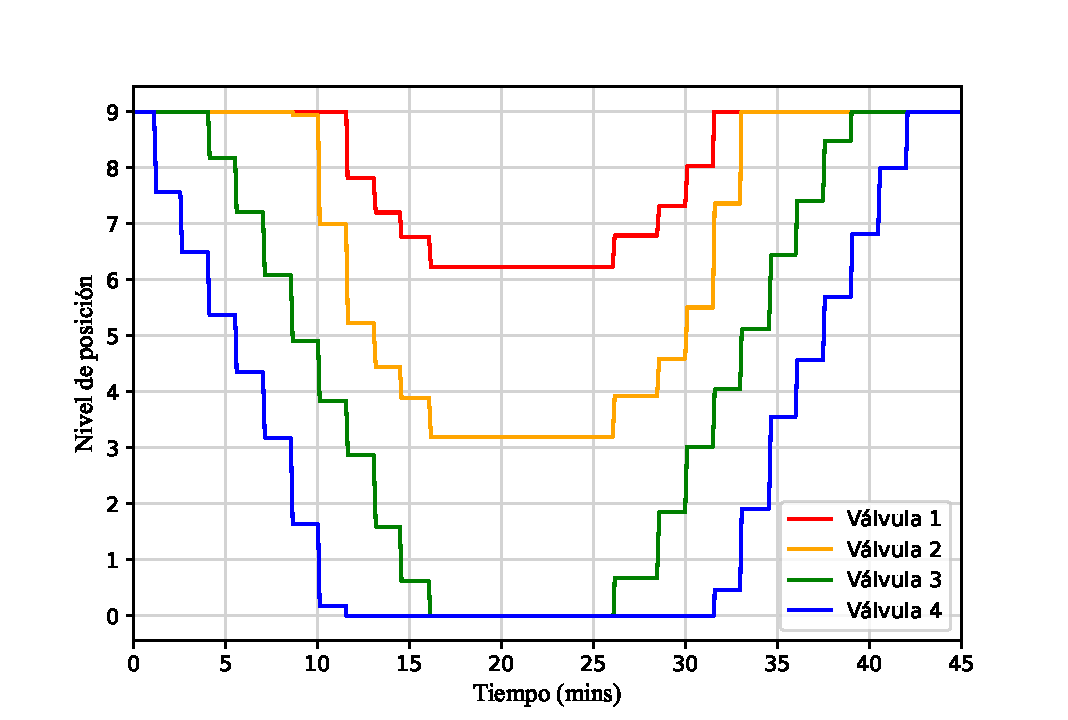
\includegraphics[width=0.75\textwidth]{content/figures/sim1_valvulas_control.pdf}
  \caption{\textit{Gráfica 3} - Posición de las válvulas de admisión de vapor a la turbina.}
  \label{fig:sim1_valvulas_control}
\end{figure}

\begin{figure}[h]
  \centering
  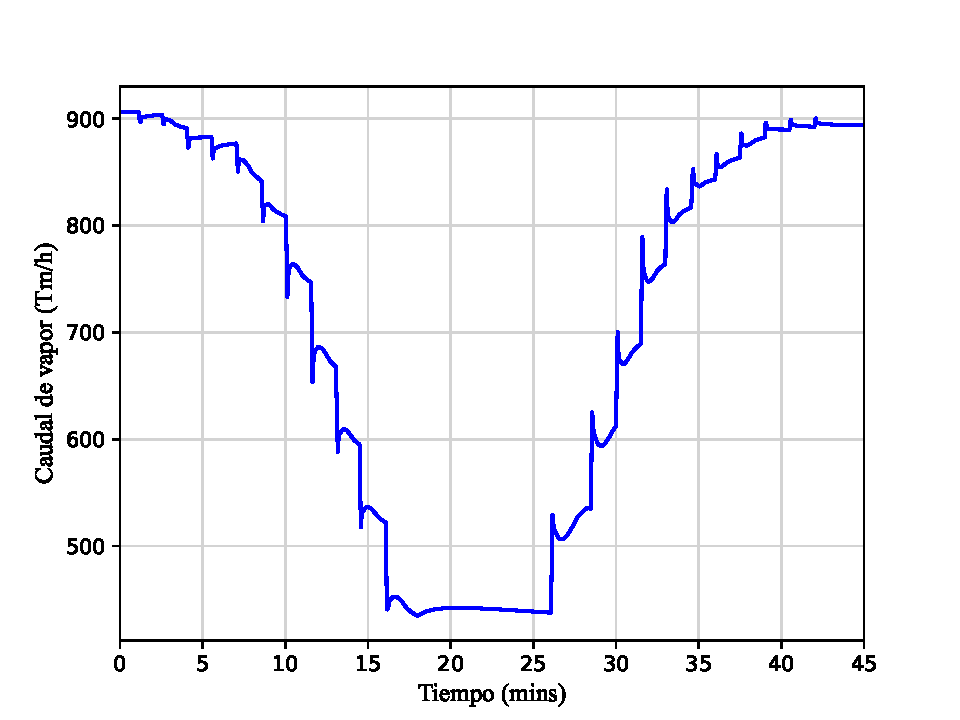
\includegraphics[width=0.75\textwidth]{content/figures/sim1_vapor.pdf}
  \caption{\textit{Gráfica 4} - Caudal de vapor que entra a la turbina.}
  \label{fig:sim1_vapor}
\end{figure}

\underline{Observaciones:} Al cerrar las válvulas de regulación, disminuye el caudal ---y, por tanto, el gasto másico--- de vapor que entra en la turbina. La gran influencia del caudal de vapor sobre la potencia generada por la turbina se pone de manifiesto al observar que el comportamiento de las curvas de \textit{caudal de vapor} y de \textit{potencia del generador} es idéntico.

\begin{figure}[!h]
  \centering
  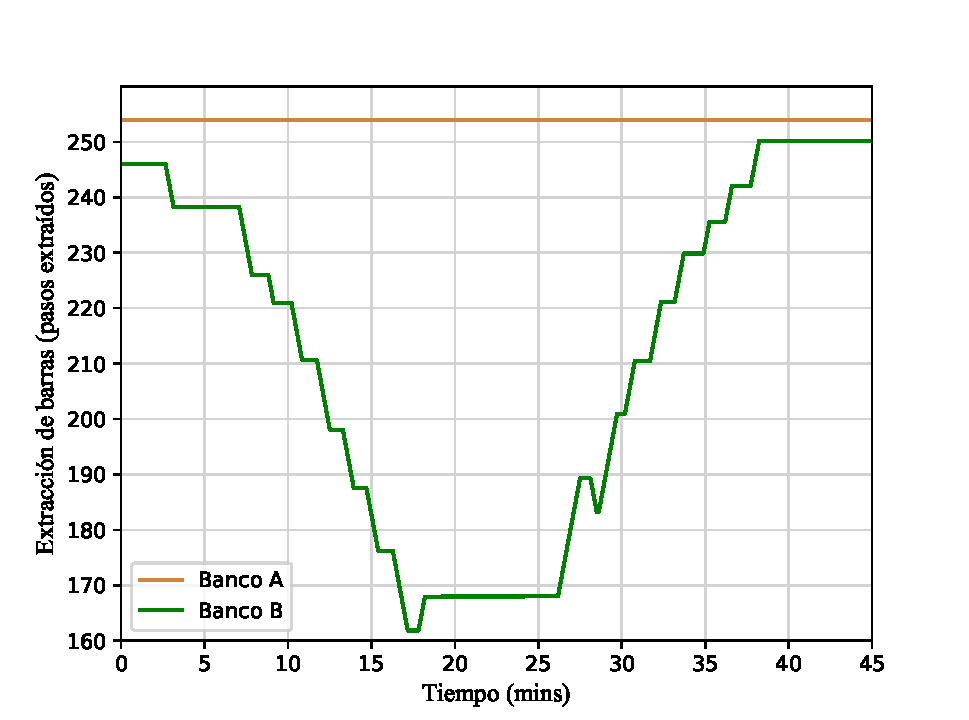
\includegraphics[width=0.8\textwidth]{content/figures/sim1_barras_control.pdf}
  \caption{\textit{Gráfica 5} - Inserción de las barras de control en el núcleo de reactor.}
  \label{fig:sim1_barras_control}
\end{figure}

\newpage
\underline{Cuestión gráfica 5:} El sistema de control automático del reactor responde a las diferencias superiores a 0.83ºC entre la $T_{med}$ y la $T_{ref}$. Si la $T_{med}$ supera en 0,83ºC a la $T_{ref}$, se insertan las barras de control, insertando así reactividad negativa, pues el primario está dando una potencia mayor que la demandada por el secundario. En el caso contrario, se extraen las barras de control. De esta manera, se ajusta la temperatura real con la de referencia, ajustando al mismo tiempo la potencia nuclear con la nueva potencia demandada en la turbina.

\underline{Observación adicional:} Comparando esta curva de inserción de barras con la de la \textit{potencia nuclear}, se observa que tienen un comportamiento prácticamente idéntico, lo que refleja la rápida respuesta del sistema automático de inserción de barras de control.

\begin{figure}[h]
  \centering
  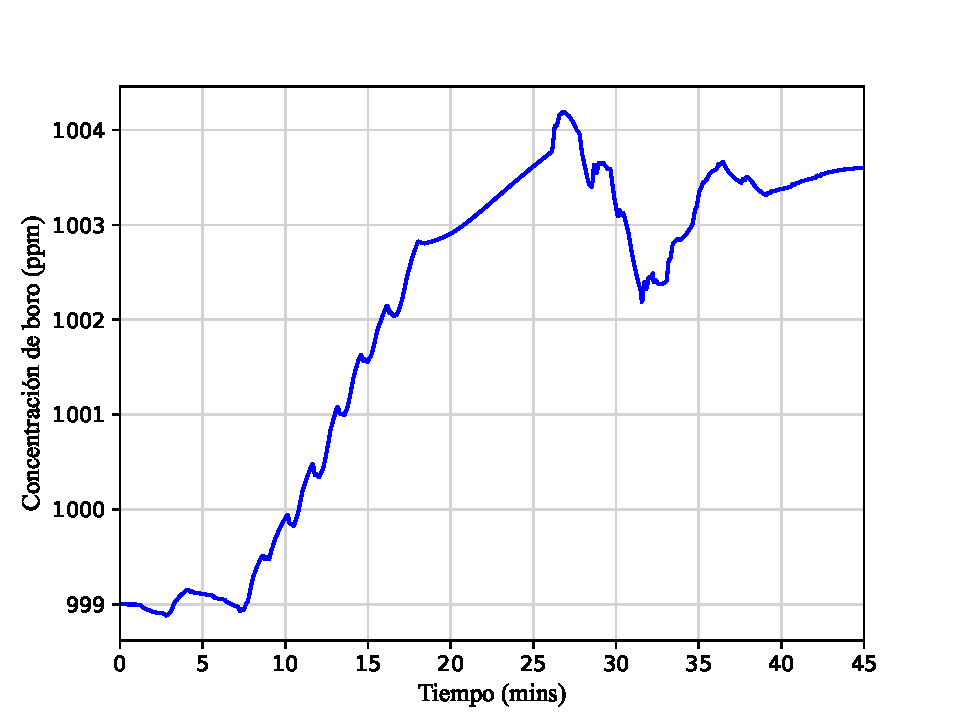
\includegraphics[width=0.75\textwidth]{content/figures/sim1_boro.pdf}
  \caption{\textit{Gráfica 6} - Variación en la concentración de boro en el circuito primario.}
  \label{fig:sim1_boro}
\end{figure}

\underline{Cuestión gráfica 6:} La inserción de barras de  control es muy efectiva, pero provoca una distorsión en la distribución del flujo neutrónico y, por tanto, de la potencia, ya que se agota más el combustible en la parte inferior del reactor que en la parte superior, por donde se insertan dichas barras en el caso de los \acrshortpl{pwr}. La inyección de ácido bórico es especialmente interesante para compensar estos desequilibrios en la distribución del flujo a lo largo del núcleo del reactor.

\underline{Observación adicional:} La curva demuestra el lento aumento en la concentración de boro cuando así se requiere, pues tarda una cantidad considerable de tiempo en aumentar muy ligeramente su concentración.

\begin{figure}[h]
  \centering
  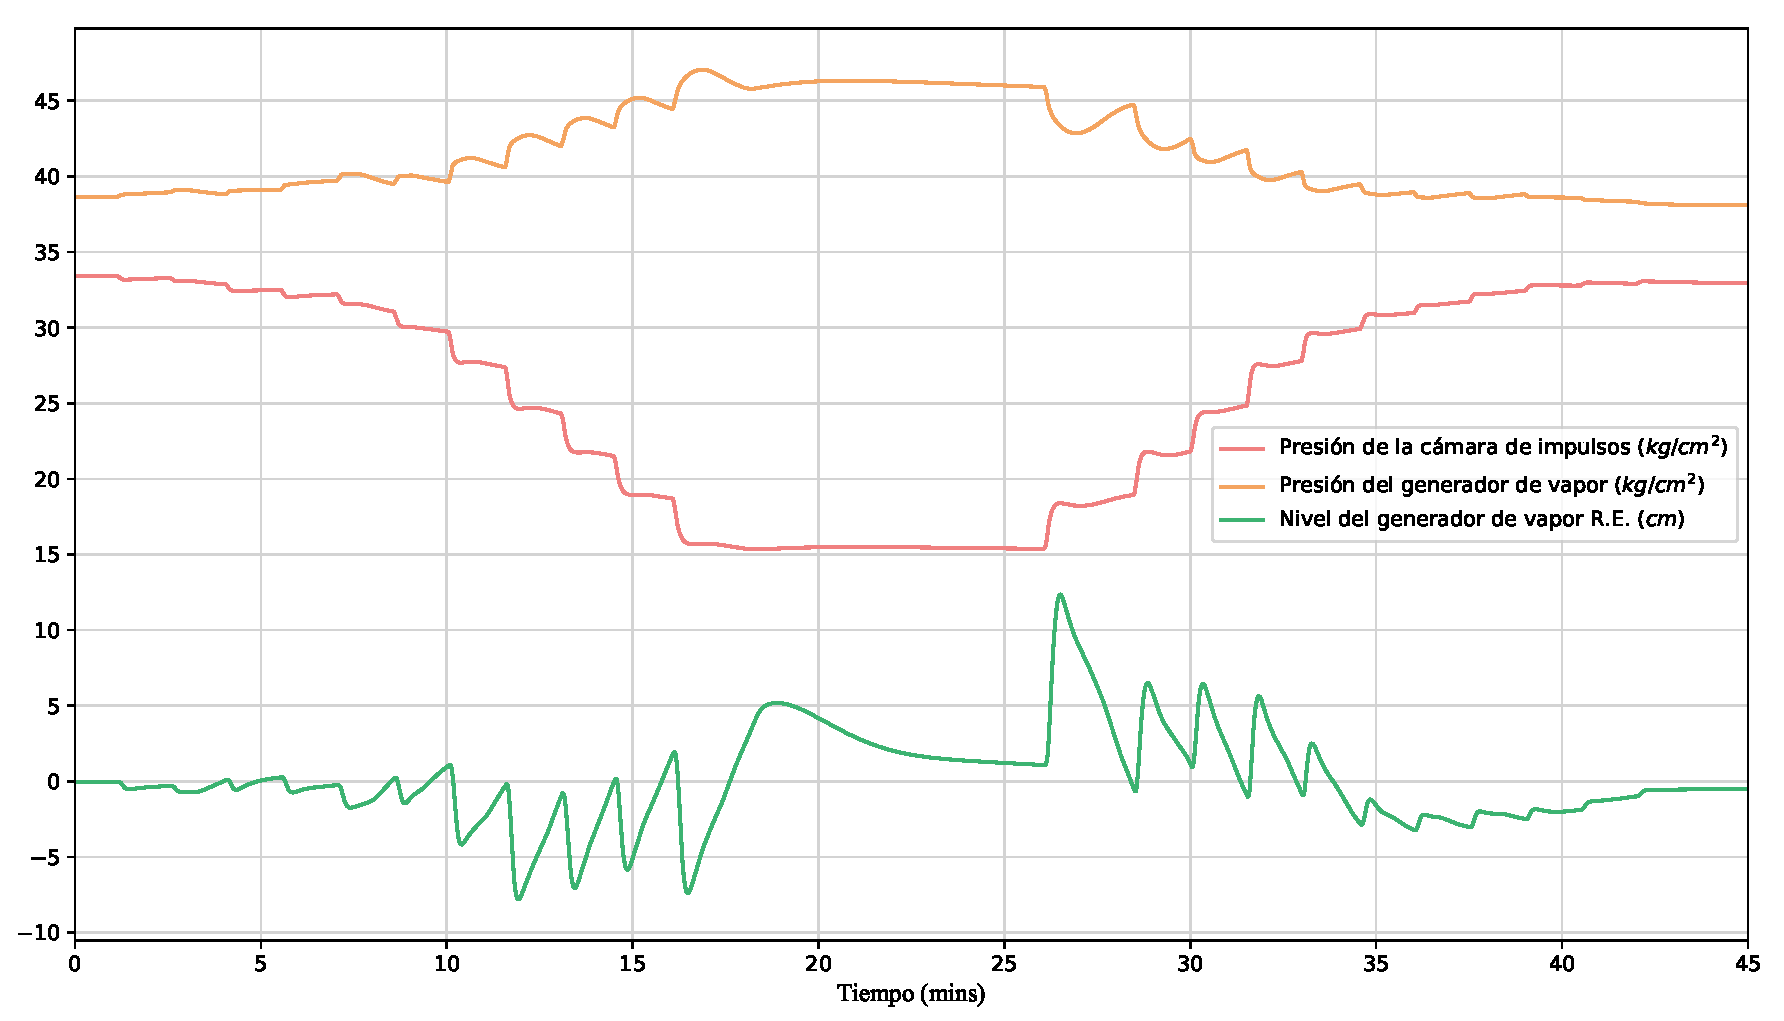
\includegraphics[width=0.96\textwidth]{content/figures/sim1_gen_vapor_camara_imp.pdf}
  \caption{\textit{Gráfica 7} - Propiedades del generador de vapor y la cámara de impulsos.}
  \label{fig:sim1_gen_vapor_camara_imp}
\end{figure}

\begin{figure}[!h]
  \centering
  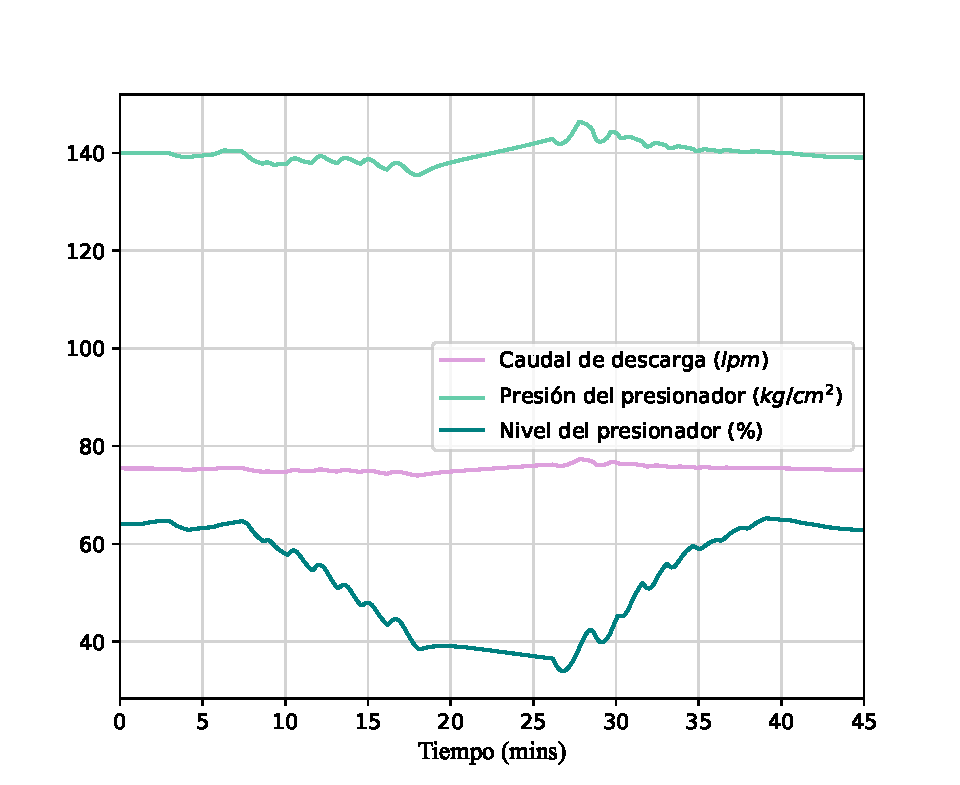
\includegraphics[width=0.8\textwidth]{content/figures/sim1_presionador.pdf}
  \caption{\textit{Gráfica 8} - Propiedades del presionador.}
  \label{fig:sim1_presionador}
\end{figure}

\underline{Cuestión gráficas 7 y 8:} Al ser esta una cuestión más amplia, se aprovecha para explicar el comportamiento general del sistema, justificando así las tendencias de las \textit{gráficas 7 y 8}. Sin embargo, no es necesario que la explicación del alumno sea de esta extensión.

Al cerrar parcialmente las válvulas de admisión de vapor a la turbina de alta presión, a parte de disminuir el gasto de vapor entrante a la turbina, el vapor sufre un proceso de laminación, disminuyendo su presión en el interior de la cámara de impulsos\footnote{Es la cámara de admisión de vapor al primer escalonamiento de la turbina.} ---tal y como se muestra en la curva roja de la \textit{gráfica 7}---. De esta manera, disminuye el salto entálpico y, por tanto, la potencia generada por la turbina. Al disminuir la potencia, disminuye la ($T_{ref}$) asociada al secundario.

Asimismo, al disminuir el gasto de vapor entrante a la turbina, como inmediatamente no se ha actuado sobre ningún otro componente, en el generador de vapor se sigue produciendo la misma cantidad de vapor, lo que provoca una acumulación o ``saturación'' del mismo hasta las válvulas de entrada a la turbina, aumentando así la presión en la admisión (aguas arriba de las válvulas) y en el generador de vapor ---tal y como se muestra en la curva naranja de la \textit{gráfica 7}---. Al ser el generador de vapor un sistema en equilibrio líquido-vapor, el incremento de presión conlleva un incremento de temperatura.

Al detectarse variaciones cada vez más grandes en el nivel del generador de vapor ---tal y como se aprecia en la curva verde de la \textit{gráfica 7}---, el sistema de control del nivel ordena el cierre de válvula de entrada al generador de vapor (válvula LCV-1947), disminuyendo el caudal de agua de alimentación. De esta manera, se consigue estabilizar la presión del generador de vapor, aunque siga siendo mayor a la nominal. 

Como consecuencia del calentamiento del circuito secundario y la reducción del caudal de agua de alimentación, la refrigeración del primario es menos efectiva, lo que provoca un aumento de la $T_{med}$ del primario. Tal y como se ha comentado anteriormente, al superar en 0.83ºC la $T_{ref}$, el sistema de control inserta automáticamente las barras de control, disminuyendo así la $T_{med}$ y la potencia del reactor. Estas subidas y bajadas de la $T_{med}$ del primario, provocan oscilaciones en la presión y en el nivel del presionador, así como en el caudal de descarga ---tal y como se observa en la \textit{gráfica 8}---:

\begin{itemize}
  \item En las fases de aumento de la $T_{med}$, aumenta consecuentemente la presión en el presionador. Asimismo, el agua se dilata y sube el nivel del presionador. El control de nivel del presionador ordena automáticamente al sistema de control volumétrico que aumente el caudal de descarga con el fin de disminuir dicho nivel al nuevo valor fijado por la $T_{med}$. 
  \item En las fases de disminución de la $T_{med}$ por el avance en la inserción de las barras de control, ocurre lo contrario: al disminuir la presión del presionador, el agua se contrae y es necesario disminuir el caudal de descarga.
\end{itemize}

Estos aumentos y disminuciones de la presión del presionador pueden provocar la actuación automática de la ducha principal (válvula PCV-400A) y de los calentadores, respectivamente.

Por último, es importante remarcar que el análisis realizado para responder a esta cuestión se ha hecho para el caso de la bajada de carga, pero todos los fenómenos descritos ocurren exactamente al revés cuando se produce una subida de potencia, tal y como se observa en las gráficas obtenidas.

\underline{Tabla de resultados y cuestión SMRs}: Tal y como se ha comentado en el \textit{procedimiento} de la simulación (apartado \ref{procedimiento}), la Central Nuclear de Zorita permite una correcta adaptación automática a variaciones de potencia entre el 15 y el 100\% cuando se emplean tasas de variación de carga de alrededor del 3\%/min, permitiendo llevar a cabo una maniobra considerablemente rápida de seguimiento de carga. Los valores obtenidos en la \textit{tabla de resultados} (tabla \ref{tab:resultados_simulacion1_solucion}) y las curvas de potencia de la \textit{gráfica de la simulación de larga duración} (figura \ref{fig:sim2_potencias}) lo demuestran. De hecho, en esta última gráfica obtenida en el \acrshort{sgiz} (figura \ref{fig:sim2_potencias}), se oberva una maniobra de seguimiento de carga análoga ---pero con mayores tasas de variación de potencia--- a la gráfica obtenida en un estudio real sobre el seguimiento de carga con \acrlongpl{smr} (figura \ref{fig:seguimiento de carga_smr}). Además, tal y como se observa en la tabla de \textit{capacidad de seguimiento de carga de los \acrshortpl{smr}} (tabla \ref{tab:capacidad_seguimiento_de_carga_smrs2}), los \acrshortpl{smr} de tipo \acrshort{pwr} tienen aproximadamente el mismo rango permitido y las mismas rampas de potencia, por lo que se puede decir que \textbf{el \acrshort{sgiz} permite realizar una aproximación realista de lo que sería una operación de seguimiento de carga en un \acrshort{smr} de tipo \acrshort{pwr}}, como lo es el AP300, por ejemplo. Aún así, es importante destacar que, a diferencia de las centrales nucleares convencionales ---o de la misma central de José Cabrera---, destinadas prinicpalmente a operar como centrales base, los \acrshortpl{smr} se diseñan con el objetivo de facilitar la adaptación a redes eléctricas con fuertes penetraciones de energías renovables intermitentes. Por tanto, una maniobra de seguimiento de carga como esta supone forzar considerablemente la central nuclear en cuestión ---tal y como demuestran las inestabilidades de la gráfica \ref{fig:sim2_potencias} a potencias muy bajas---, mientras que los pequeños reactores modulares se conciben para realizar a menudo esta operación sin que ello supongo ninguna desestabilización del sistema ni ningún daño para sus equipos.

\begin{table}[h]
  \centering
  \resizebox{1\textwidth}{!}{%
  \begin{tabular}{|c|c|c|c|c|c|c|}
    \hline
    \rowcolor[HTML]{ECF4FF} 
    \textbf{\begin{tabular}[c]{@{}c@{}}Potencia inicial\\ (MWe \\ generados\\  y \% nuclear)\end{tabular}} &
      \textbf{\begin{tabular}[c]{@{}c@{}}Potencia \\ intermedia\\ (MWe generados\\  y \% nuclear)\end{tabular}} &
      \textbf{\begin{tabular}[c]{@{}c@{}}Duración \\ bajada\\ de potencia\\ (min)\end{tabular}} &
      \textbf{\begin{tabular}[c]{@{}c@{}}Rampa media\\ de potencia \\ en la bajada\\ (\%/min)\end{tabular}} &
      \textbf{\begin{tabular}[c]{@{}c@{}}Potencia final\\ (MWe \\ generados\\  y \% nuclear)\end{tabular}} &
      \textbf{\begin{tabular}[c]{@{}c@{}}Duración \\ subida\\ de potencia \\ (min)\end{tabular}} &
      \textbf{\begin{tabular}[c]{@{}c@{}}Rampa media \\ de potencia\\ en la subida \\ (\%/min)\end{tabular}} \\ \hline
    \cellcolor[HTML]{FFFFFF}\begin{tabular}[c]{@{}c@{}}142,65 MWe\\ 96,3\%\tablefootnote{Por un error de diseño en la Central Nuclear de Zorita, el 100\% de turbina corresponde al 96,3\% de potencia del reactor.} nuclear\end{tabular} &
      \begin{tabular}[c]{@{}c@{}}75,5 MWe\\ 47,5\% nuclear\end{tabular} &
      16,5 mins &
      2,96 \%/min &
      \begin{tabular}[c]{@{}c@{}}141,1 MWe\\ 95,3\% nuclear\end{tabular} &
      19 mins &
      2,52 \%/min \\ \hline
    \end{tabular}
  }
  \caption{Resultados de la maniobra de seguimiento de carga realizada en el \acrshort{sgiz} el 12 de abril de 2024.}
  \label{tab:resultados_simulacion1_solucion}
  \end{table}

% ---------------- Segundo anexo --------------- %
\newpage
\subsection{Anexo II} \label{sec:anexo2}

%%%%%%%%%%%%%%%%%%%%%%%%%%%%%%%%%%%%%%%%%%%%%%%%%%